\documentclass[../main]{subfiles}
\begin{document}

\graphicspath{{../figures/chap1/}}

\section{背景}
\label{sec:intro_background}
台風や梅雨前線,線状降水帯による大雨,地震,噴火などの自然災害は土砂災害を誘発する場合が多く,自然災害が多発している日本では土砂災害も頻発している\citeja{cao2014main1-1-4-3}.
2011年から2021年における日本での土砂災害発生件数を\reffig{fig:num_landslides}に示す.
グラフが示すように,日本における土砂災害の年間平均発生件数は\numcomma{1000}件以上となっており,人命や家屋に対する被害も甚大になっている.
特に2018年には平成30年7月豪雨や北海道胆振東部地震などの影響により,当時の過去10年の平均発生件数の3倍以上となる\numcomma{3459}件もの土砂災害が発生した\citeja{mlit2021}.
また,2021年8月には九州地方や中国地方で線状降水帯が発生するなど,西日本を中心に各地で大雨となり,平年の8月を大きく上回る448件の土砂災害が発生した\citeja{mlit2022landslide}.

\vspace{9\zh}
\begin{figure}[h]
    \centering
    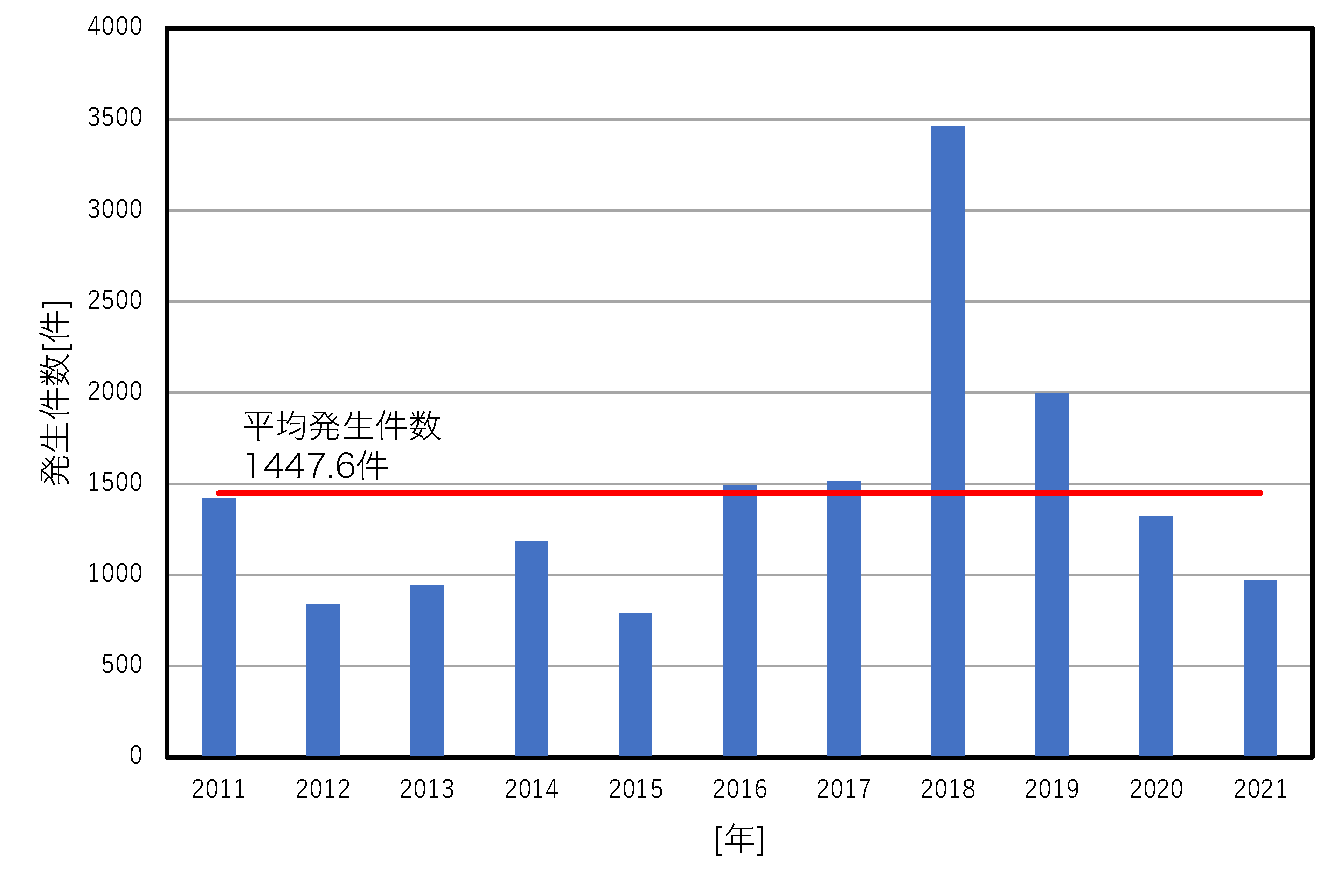
\includegraphics[keepaspectratio, width=0.8\linewidth]{num_year_landslides.pdf}
    \caption{土砂災害の発生件数(\protect\citeja{mlit2022landslide}を基に作成)}
    \label{fig:num_landslides}
\end{figure}
\clearpage

災害現場では土砂災害の再発や土木や建造物の倒壊といった二次災害の危険性があり,作業員の立ち入りには危険が伴う\citeja{Hino2010}.
そのため,復旧作業においては二次災害を防ぐために操縦者が建設機械に搭乗せず,現場の映像を見ながら建設機械を遠隔操作する無人化施工が利用されることもある\citeja{Motegi2016}\citeen{Kiribayashi2018}.
また,建設機械が走行する場所が水分を多く含む軟弱な地盤だと,地盤が建設機械を支えきれずに建設機械が沈み込み,スタックしたり,場合によっては転倒したりする可能性もある\citeja{Tanaka2009}.
スタックや転倒が起きると,その建設機械を復帰させるために他の作業が遅延・中断してしまい,復旧作業に遅れが生じる.
建設機械に人が搭乗し,操作しているときと異なり,無人化施工では車体の傾きや振動数などの微小な変化を搭乗者の体性感覚として知覚することができない\citeja{Shigematsu2017}.
そのため,遠隔操作する操縦者が危険性を判断できず,スタックや転倒の回避を行うことが困難になる.
そこで,地盤強度をあらかじめ調査し,建設機械が走破可能かどうかを判定した上で,走破不可能な場所を回避して走行する方法が考えられる.
土砂災害現場では異なる特性を持つ複数の土砂が堆積していることもあるため\citeja{Doshida2018},一部分だけではなく災害現場全体に対して調査を行う必要がある.
加えて,建設機械を投入する前に調査を行う必要があるので,迅速さも求められる.

\end{document}